\documentclass[10pt,fleqn]{article} % Default font size and left-justified equations
\usepackage[%
    pdftitle={CIN : Cinématique du solide},
    pdfauthor={Xavier Pessoles}]{hyperref}

%%%%%%%%%%%%%%%%%%%%%%%%%%%%%%%%%%%%%%%%%
% Original author:
% Mathias Legrand (legrand.mathias@gmail.com) with modifications by:
% Vel (vel@latextemplates.com)
% License:
% CC BY-NC-SA 3.0 (http://creativecommons.org/licenses/by-nc-sa/3.0/)
%%%%%%%%%%%%%%%%%%%%%%%%%%%%%%%%%%%%%%%%%

%----------------------------------------------------------------------------------------
%	VARIOUS REQUIRED PACKAGES AND CONFIGURATIONS
%----------------------------------------------------------------------------------------

\usepackage[top=2.5cm,bottom=2cm,left=2cm,right=2cm,headsep=40pt,a4paper]{geometry} % Page margins

\usepackage{graphicx} % Required for including pictures
\graphicspath{{images/}} % Specifies the directory where pictures are stored

\usepackage{lipsum} % Inserts dummy text

\usepackage{tikz} % Required for drawing custom shapes

\usepackage[french]{babel} % English language/hyphenation
\frenchbsetup{StandardLists=true} % Pour éviter la collision babel enumitem pour les listes

\usepackage{enumitem} % Customize lists
\setlist{nolistsep} % Reduce spacing between bullet points and numbered lists

\usepackage{booktabs} % Required for nicer horizontal rules in tables

\usepackage{xcolor} % Required for specifying colors by name
%\definecolor{ocre}{RGB}{243,102,25} % Define the orange color used for highlighting throughout the book
 \definecolor{ocre}{RGB}{49,133,156} % Couleur ''bleue''
\definecolor{violetf}{RGB}{112,48,160} % Couleur ''violet''
\usepackage{enumitem}
\usepackage{pifont} % Pour les dinglist
%----------------------------------------------------------------------------------------
%	FONTS
%----------------------------------------------------------------------------------------

\usepackage{avant} % Use the Avantgarde font for headings
%\usepackage{times} % Use the Times font for headings
%\usepackage{mathptmx} % Use the Adobe Times Roman as the default text font together with math symbols from the Sym­bol, Chancery and Com­puter Modern fonts
\usepackage[adobe-utopia]{mathdesign}
\usepackage{microtype} % Slightly tweak font spacing for aesthetics
\usepackage[utf8]{inputenc} % Required for including letters with accents
\usepackage[T1]{fontenc} % Use 8-bit encoding that has 256 glyphs

%----------------------------------------------------------------------------------------
%	BIBLIOGRAPHY AND INDEX
%----------------------------------------------------------------------------------------

\usepackage[style=alphabetic,citestyle=numeric,sorting=nyt,sortcites=true,autopunct=true,babel=hyphen,hyperref=true,abbreviate=false,backref=true,backend=biber]{biblatex}
\addbibresource{bibliography.bib} % BibTeX bibliography file
\defbibheading{bibempty}{}

\usepackage{calc} % For simpler calculation - used for spacing the index letter headings correctly
\usepackage{makeidx} % Required to make an index
\makeindex % Tells LaTeX to create the files required for indexing

%----------------------------------------------------------------------------------------
%	MAIN TABLE OF CONTENTS
%----------------------------------------------------------------------------------------

\usepackage{titletoc} % Required for manipulating the table of contents

\setcounter{tocdepth}{2}     % Dans la table des matieres
\setcounter{secnumdepth}{2}

\contentsmargin{0cm} % Removes the default margin

% Part text styling
\titlecontents{part}[0cm]
{\addvspace{20pt}\centering\large\bfseries}
{}
{}
{}

% Chapter text styling
\titlecontents{chapter}[1.25cm] % Indentation
{\addvspace{12pt}\large\sffamily\bfseries} % Spacing and font options for chapters
{\color{ocre!60}\contentslabel[\Large\thecontentslabel]{1.25cm}\color{ocre}} % Chapter number
{\color{ocre}}  
{\color{ocre!60}\normalsize\;\titlerule*[.5pc]{.}\;\thecontentspage} % Page number

% Section text styling
\titlecontents{section}[1.25cm] % Indentation
{\addvspace{3pt}\sffamily\bfseries} % Spacing and font options for sections
{\color{ocre!60}\contentslabel[\thecontentslabel]{1.25cm} \color{ocre}} % Section number
{\color{ocre}}
{\hfill\color{ocre!60}\thecontentspage} % Page number
[]

% Subsection text styling
\titlecontents{subsection}[1.25cm] % Indentation
{\addvspace{1pt}\sffamily\small} % Spacing and font options for subsections
{\contentslabel[\thecontentslabel]{1.25cm}} % Subsection number
{}
{\ \titlerule*[.5pc]{.}\;\thecontentspage} % Page number
[]

% List of figures
\titlecontents{figure}[0em]
{\addvspace{-5pt}\sffamily}
{\thecontentslabel\hspace*{1em}}
{}
{\ \titlerule*[.5pc]{.}\;\thecontentspage}
[]

% List of tables
\titlecontents{table}[0em]
{\addvspace{-5pt}\sffamily}
{\thecontentslabel\hspace*{1em}}
{}
{\ \titlerule*[.5pc]{.}\;\thecontentspage}
[]

%----------------------------------------------------------------------------------------
%	MINI TABLE OF CONTENTS IN PART HEADS
%----------------------------------------------------------------------------------------

% Chapter text styling
\titlecontents{lchapter}[0em] % Indenting
{\addvspace{15pt}\large\sffamily\bfseries} % Spacing and font options for chapters
{\color{ocre}\contentslabel[\Large\thecontentslabel]{1.25cm}\color{ocre}} % Chapter number
{}  
{\color{ocre}\normalsize\sffamily\bfseries\;\titlerule*[.5pc]{.}\;\thecontentspage} % Page number

% Section text styling
\titlecontents{lsection}[0em] % Indenting
{\sffamily\small} % Spacing and font options for sections
{\contentslabel[\thecontentslabel]{1.25cm}} % Section number
{}
{}

% Subsection text styling
\titlecontents{lsubsection}[.5em] % Indentation
{\normalfont\footnotesize\sffamily} % Font settings
{}
{}
{}

%----------------------------------------------------------------------------------------
%	PAGE HEADERS
%----------------------------------------------------------------------------------------

\usepackage{fancyhdr} % Required for header and footer configuration



\pagestyle{fancy}
 \renewcommand{\headrulewidth}{0pt}
 \fancyhead{}
 \fancyhead[L]{%
 \noindent\begin{minipage}[c]{2.6cm}%
 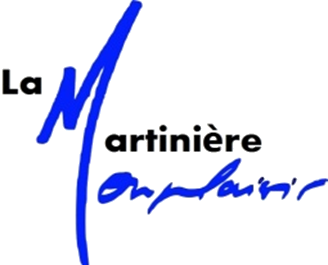
\includegraphics[width=2cm]{png/logo_lycee.png}%
 \end{minipage}}

\fancyhead[C]{\rule{8cm}{.5pt}}

 \fancyhead[R]{%
 \noindent\begin{minipage}[c]{3cm}
 \begin{flushright}
 \footnotesize{\textit{\textsf{\xxtete}}}%
 \end{flushright}
 \end{minipage}
}


\fancyfoot[C]{\rule{12cm}{.5pt}}
\renewcommand{\footrulewidth}{0.2pt}
\fancyfoot[C]{\footnotesize{\bfseries \thepage}}
\fancyfoot[L]{ 
\begin{minipage}[c]{.2\linewidth}
\noindent\footnotesize{{\xxauteur}}
\end{minipage}}


\fancyfoot[R]{\footnotesize{\xxpied}
\ifthenelse{\isodd{\value{page}}}{
\begin{tikzpicture}[overlay]
\node[shape=rectangle, 
      rounded corners = .25 cm,
	  draw= ocre,
	  line width=2pt, 
	  fill = ocre!10,
	  minimum width  = 2.5cm,
	  minimum height = 3cm,] at (\xxposongletx,\xxposonglety) {};
\node at (\xxposonglettext,\xxposonglety) {\rotatebox{90}{\textbf{\large\color{ocre}{\xxonglet}}}};
%{};
\end{tikzpicture}}{}
}
%
%
%
% Removes the header from odd empty pages at the end of chapters
\makeatletter
\renewcommand{\cleardoublepage}{
\clearpage\ifodd\c@page\else
\hbox{}
\vspace*{\fill}
\thispagestyle{empty}
\newpage
\fi}

\fancypagestyle{plain}{%
\fancyhf{} % vide l’en-tête et le pied~de~page.
%\fancyfoot[C]{\bfseries \thepage} % numéro de la page en cours en gras
% et centré en pied~de~page.
\fancyfoot[R]{\footnotesize{\xxpied}}
\fancyfoot[C]{\rule{12cm}{.5pt}}
\renewcommand{\footrulewidth}{0.2pt}
\fancyfoot[C]{\footnotesize{\bfseries \thepage}}
\fancyfoot[L]{ 
\begin{minipage}[c]{.2\linewidth}
\noindent\footnotesize{{\xxauteur}}
\end{minipage}}}



%----------------------------------------------------------------------------------------
%	THEOREM STYLES
%----------------------------------------------------------------------------------------

% Conflit avec la police adobe
%\usepackage{amsmath,amsfonts,amssymb,amsthm} % For math equations, theorems, symbols, etc
\usepackage{amsmath,amsthm}

\newcommand{\intoo}[2]{\mathopen{]}#1\,;#2\mathclose{[}}
\newcommand{\ud}{\mathop{\mathrm{{}d}}\mathopen{}}
\newcommand{\intff}[2]{\mathopen{[}#1\,;#2\mathclose{]}}
%\newtheorem{notation}{Notation}[chapter]
\newtheorem{notation}{Notation}[section]

% Boxed/framed environments
\newtheoremstyle{ocrenumbox}% % Theorem style name
{0pt}% Space above
{0pt}% Space below
{\normalfont}% % Body font
{}% Indent amount
{\small\bf\sffamily\color{ocre}}% % Theorem head font
{\;}% Punctuation after theorem head
{0.25em}% Space after theorem head
{\small\sffamily\color{ocre}\thmname{#1}\nobreakspace\thmnumber%{\@ifnotempty{#1}{}\@upn{#2}}% Theorem text (e.g. Theorem 2.1)
\thmnote{\nobreakspace\the\thm@notefont\sffamily\bfseries\color{black}---\nobreakspace#3.}} % Optional theorem note
\renewcommand{\qedsymbol}{$\blacksquare$}% Optional qed square


% Boite pour les corriges
\newtheoremstyle{correctionbox}% % Theorem style name
{0pt}% Space above
{0pt}% Space below
{\normalfont}% % Body font
{}% Indent amount
{\small\bf\sffamily\color{violet}}% % Theorem head font
{\;}% Punctuation after theorem head
{0.25em}% Space after theorem head
{\small\sffamily\color{ocre}\thmname{#1}\nobreakspace\thmnumber%{\@ifnotempty{#1}{}\@upn{#2}}% Theorem text (e.g. Theorem 2.1)
\thmnote{\nobreakspace\the\thm@notefont\sffamily\bfseries\color{black}---\nobreakspace#3.}} % Optional theorem note
\renewcommand{\qedsymbol}{$\blacksquare$}% Optional qed square



\newtheoremstyle{blacknumex}% Theorem style name
{5pt}% Space above
{5pt}% Space below
{\normalfont}% Body font
{} % Indent amount
{\small\bf\sffamily}% Theorem head font
{\;}% Punctuation after theorem head
{0.25em}% Space after theorem head
{\small\sffamily{\tiny\ensuremath{\blacksquare}}\nobreakspace\thmname{#1}\nobreakspace\thmnumber%{\@ifnotempty{#1}{}\@upn{#2}}% Theorem text (e.g. Theorem 2.1)
\thmnote{\nobreakspace\the\thm@notefont\sffamily\bfseries---\nobreakspace#3.}}% Optional theorem note

\newtheoremstyle{blacknumbox} % Theorem style name
{0pt}% Space above
{0pt}% Space below
{\normalfont}% Body font
{}% Indent amount
{\small\bf\sffamily}% Theorem head font
{\;}% Punctuation after theorem head
{0.25em}% Space after theorem head
{\small\sffamily\thmname{#1}\nobreakspace%\thmnumber{\@ifnotempty{#1}{}\@upn{#2}}% Theorem text (e.g. Theorem 2.1)
\thmnote{\nobreakspace\the\thm@notefont\sffamily\bfseries---\nobreakspace#3.}}% Optional theorem note

% Non-boxed/non-framed environments
\newtheoremstyle{ocrenum}% % Theorem style name
{5pt}% Space above
{5pt}% Space below
{\normalfont}% % Body font
{}% Indent amount
{\small\bf\sffamily\color{ocre}}% % Theorem head font
{\;}% Punctuation after theorem head
{0.25em}% Space after theorem head
{\small\sffamily\color{ocre}\thmname{#1}\nobreakspace\thmnumber{\@ifnotempty{#1}{}\@upn{#2}}% Theorem text (e.g. Theorem 2.1)
\thmnote{\nobreakspace\the\thm@notefont\sffamily\bfseries\color{black}---\nobreakspace#3.}} % Optional theorem note
\renewcommand{\qedsymbol}{$\blacksquare$}% Optional qed square
\makeatother

% Environnement pour les titres de parties
\newtheoremstyle{partiebox} 
{0pt}% Space above
{0pt}% Space below
{\normalfont}% Body font
{}% Indent amount
{\small\bf\sffamily}% Theorem head font
{\;}% Punctuation after theorem head
{0.25em}% Space after theorem head




% Defines the theorem text style for each type of theorem to one of the three styles above
\newcounter{dummy} 
\numberwithin{dummy}{section}
\theoremstyle{ocrenumbox}
%\newtheorem{theoremeT}[dummy]{Théorème}
\newtheorem{theoremeT}[dummy]{Théorème}
\newtheorem{resultatT}[dummy]{Résultat}
\newtheorem{objectifT}[dummy]{Objectif}
%\newtheorem{problem}{Problem}[chapter]
\newtheorem{problem}{Problem}[section]
%\newtheorem{exerciseT}{Exercise}[chapter]
\newtheorem{exerciseT}{Exercice}[section]

\theoremstyle{blacknumex}
%\newtheorem{exampleT}{Example}[chapter]
\newtheorem{exempleT}{Exemple}[section]
\theoremstyle{blacknumbox}
%\newtheorem{vocabulary}{Vocabulary}[chapter]
\newtheorem{vocabulary}{Vocabulaire}[section]
%\newtheorem{definitionT}{Definition}[section]
\newtheorem{definitionT}{Définition}[section]
\newtheorem{corollaryT}[dummy]{Corollaire}
\newtheorem{hypoT}{Hypothèse(s)}

\theoremstyle{ocrenum}
\newtheorem{proposition}[dummy]{Proposition}

\theoremstyle{partiebox}
\newtheorem{titrepartieT}[]{}
\newtheorem{titrechapitreT}[]{}

\theoremstyle{correctionbox}
\newtheorem{correctionT}[dummy]{\color{violet}{Correction}}

%----------------------------------------------------------------------------------------
%	DEFINITION OF COLORED BOXES
%----------------------------------------------------------------------------------------

\RequirePackage[framemethod=tikz]{mdframed} % Required for creating the theorem, definition, exercise and corollary boxes

% Theorem box
\newmdenv[skipabove=7pt,
skipbelow=7pt,
backgroundcolor=ocre!10,
linecolor=ocre,
innerleftmargin=5pt,
innerrightmargin=5pt,
innertopmargin=5pt,
leftmargin=0cm,
rightmargin=0cm,
innerbottommargin=5pt]{tBox}


% Correction
\newmdenv[skipabove=7pt,
skipbelow=7pt,
backgroundcolor=violet!10,
linecolor=violet,
innerleftmargin=5pt,
innerrightmargin=5pt,
innertopmargin=5pt,
leftmargin=0cm,
rightmargin=0cm,
innerbottommargin=5pt]{coBox}


% Exercise box	  
\newmdenv[skipabove=7pt,
skipbelow=7pt,
rightline=false,
leftline=true,
topline=false,
bottomline=false,
backgroundcolor=ocre!10,
linecolor=ocre,
innerleftmargin=5pt,
innerrightmargin=5pt,
innertopmargin=5pt,
innerbottommargin=5pt,
leftmargin=0cm,
rightmargin=0cm,
linewidth=4pt]{eBox}	

% Definition box
\newmdenv[skipabove=7pt,
skipbelow=7pt,
rightline=false,
leftline=true,
topline=false,
bottomline=false,
backgroundcolor=ocre!10,
linecolor=ocre,
innerleftmargin=5pt,
innerrightmargin=5pt,
innertopmargin=0pt,
leftmargin=0cm,
rightmargin=0cm,
linewidth=4pt,
innerbottommargin=0pt]{dBox}	

% Corollary box
\newmdenv[skipabove=7pt,
skipbelow=7pt,
rightline=false,
leftline=true,
topline=false,
bottomline=false,
linecolor=gray,
backgroundcolor=black!5,
innerleftmargin=5pt,
innerrightmargin=5pt,
innertopmargin=5pt,
leftmargin=0cm,
rightmargin=0cm,
linewidth=4pt,
innerbottommargin=5pt]{cBox}


% Hypothèses
\newmdenv[skipabove=7pt,
skipbelow=7pt,
rightline=false,
leftline=true,
topline=false,
bottomline=false,
linecolor=gray,
backgroundcolor=black!5,
innerleftmargin=5pt,
innerrightmargin=5pt,
innertopmargin=5pt,
leftmargin=0cm,
rightmargin=0cm,
linewidth=4pt,
innerbottommargin=5pt]{hyBox}


% Boite pour le titre de la partie (pBox)
\newmdenv[skipabove=7pt,
skipbelow=7pt,
rightline=true,
leftline=false,
topline=false,
bottomline=false,
linecolor=ocre,
backgroundcolor=none,
innerleftmargin=5pt,
innerrightmargin=5pt,
innertopmargin=5pt,
leftmargin=0cm,
rightmargin=0cm,
linewidth=4pt,
innerbottommargin=5pt]{pBox}

% Boite pour le titre du chapitre (chBox)
\newmdenv[skipabove=7pt,
skipbelow=7pt,
rightline=false,
leftline=true,
topline=false,
bottomline=false,
linecolor=ocre,
%backgroundcolor=black!5,
innerleftmargin=5pt,
innerrightmargin=5pt,
innertopmargin=5pt,
leftmargin=0cm,
rightmargin=0cm,
linewidth=4pt,
innerbottommargin=5pt]{chBox}


% Boite pour les exemples
\newmdenv[skipabove=7pt,
skipbelow=7pt,
rightline=false,
leftline=true,
topline=false,
bottomline=false,
linecolor=gray,
backgroundcolor=white,
innerleftmargin=5pt,
innerrightmargin=5pt,
innertopmargin=5pt,
leftmargin=0cm,
rightmargin=0cm,
linewidth=4pt,
innerbottommargin=5pt]{exBox}


% Creates an environment for each type of theorem and assigns it a theorem text style from the "Theorem Styles" section above and a colored box from above
\newenvironment{theorem}{\begin{tBox}\begin{theoremeT}}{\end{theoremeT}\end{tBox}}
\newenvironment{resultat}{\begin{tBox}\begin{resultatT}}{\end{resultatT}\end{tBox}}
\newenvironment{obj}{\begin{tBox}\begin{objectifT}}{\end{objectifT}\end{tBox}}
\newenvironment{corrige}{\begin{coBox}\begin{correctionT}}{\end{correctionT}\end{coBox}}
\newenvironment{exercise}{\begin{eBox}\begin{exerciseT}}{\hfill{\color{ocre}\tiny\ensuremath{\blacksquare}}\end{exerciseT}\end{eBox}}				  
\newenvironment{definition}{\begin{dBox}\begin{definitionT}}{\end{definitionT}\end{dBox}}	
\newenvironment{defi}{\begin{dBox}\begin{definitionT}}{\end{definitionT}\end{dBox}}	
%\newenvironment{exemple}{\begin{exempleT}}{\hfill{\tiny\ensuremath{\blacksquare}}\end{exempleT}}		
\newenvironment{corollary}{\begin{cBox}\begin{corollaryT}}{\end{corollaryT}\end{cBox}}
\newenvironment{hypo}{\begin{hyBox}\begin{hypoT}}{\end{hypoT}\end{hyBox}}	\newenvironment{exemple}{\begin{exBox}\begin{exempleT}}{\hfill{\tiny\ensuremath{\blacksquare}}\end{exempleT}\end{exBox}}	
\newenvironment{titrepartie}{\begin{pBox}\begin{titrepartieT}}{\end{titrepartieT}\end{pBox}}	
\newenvironment{titrechapitre}{\begin{chBox}\begin{titrechapitreT}}{\end{titrechapitreT}\end{chBox}}	
%----------------------------------------------------------------------------------------
%	REMARK ENVIRONMENT
%----------------------------------------------------------------------------------------

\newenvironment{remark}{\par\vspace{10pt}\small % Vertical white space above the remark and smaller font size
\begin{list}{}{
\leftmargin=35pt % Indentation on the left
\rightmargin=25pt}\item\ignorespaces % Indentation on the right
\makebox[-2.5pt]{\begin{tikzpicture}[overlay]
\node[draw=ocre!60,line width=1pt,circle,fill=ocre!25,font=\sffamily\bfseries,inner sep=2pt,outer sep=0pt] at (-15pt,0pt){\textcolor{ocre}{R}};\end{tikzpicture}} % Orange R in a circle
\advance\baselineskip -1pt}{\end{list}\vskip5pt} % Tighter line spacing and white space after remark

\newenvironment{rem}{\par\vspace{10pt}\small % Vertical white space above the remark and smaller font size
\begin{list}{}{
\leftmargin=35pt % Indentation on the left
\rightmargin=25pt}\item\ignorespaces % Indentation on the right
\makebox[-2.5pt]{\begin{tikzpicture}[overlay]
\node[draw=ocre!60,line width=1pt,circle,fill=ocre!25,font=\sffamily\bfseries,inner sep=2pt,outer sep=0pt] at (-15pt,0pt){\textcolor{ocre}{R}};\end{tikzpicture}} % Orange R in a circle
\advance\baselineskip -1pt}{\end{list}\vskip5pt} % Tighter line spacing and white space after remark


\newenvironment{warn}{\par\vspace{10pt}\small % Vertical white space above the remark and smaller font size
\begin{list}{}{
\leftmargin=35pt % Indentation on the left
\rightmargin=25pt}\item\ignorespaces % Indentation on the right
\makebox[-2.5pt]{\begin{tikzpicture}[overlay]
\node[draw=red!60,line width=1pt,circle,fill=red!25,font=\sffamily\bfseries,inner sep=2pt,outer sep=0pt] at (-15pt,0pt){\textcolor{black}{!}};\end{tikzpicture}} % Point d'exclamation dans un cercle
\advance\baselineskip -1pt}{\end{list}\vskip5pt} % Tighter line spacing and white space after remark


%----------------------------------------------------------------------------------------
%	SECTION NUMBERING IN THE MARGIN
%----------------------------------------------------------------------------------------

\makeatletter
\renewcommand{\@seccntformat}[1]{\llap{\textcolor{ocre}{\csname the#1\endcsname}\hspace{1em}}}                    
\renewcommand{\section}{\@startsection{section}{1}{\z@}
{-4ex \@plus -1ex \@minus -.4ex}
{1ex \@plus.2ex }
{\normalfont\large\sffamily\bfseries}}
\renewcommand{\subsection}{\@startsection {subsection}{2}{\z@}
{-3ex \@plus -0.1ex \@minus -.4ex}
{0.5ex \@plus.2ex }
{\normalfont\sffamily\bfseries}}
\renewcommand{\subsubsection}{\@startsection {subsubsection}{3}{\z@}
{-2ex \@plus -0.1ex \@minus -.2ex}
{.2ex \@plus.2ex }
{\normalfont\small\sffamily\bfseries}}                        
\renewcommand\paragraph{\@startsection{paragraph}{4}{\z@}
{-2ex \@plus-.2ex \@minus .2ex}
{.1ex}
{\normalfont\small\sffamily\bfseries}}

%----------------------------------------------------------------------------------------
%	PART HEADINGS
%----------------------------------------------------------------------------------------


%----------------------------------------------------------------------------------------
%	CHAPTER HEADINGS
%----------------------------------------------------------------------------------------

% \newcommand{\thechapterimage}{}%
% \newcommand{\chapterimage}[1]{\renewcommand{\thechapterimage}{#1}}%
% \def\@makechapterhead#1{%
% {\parindent \z@ \raggedright \normalfont
% \ifnum \c@secnumdepth >\m@ne
% \if@mainmatter
% \begin{tikzpicture}[remember picture,overlay]
% \node at (current page.north west)
% {\begin{tikzpicture}[remember picture,overlay]
% \node[anchor=north west,inner sep=0pt] at (0,0) {\includegraphics[width=\paperwidth]{\thechapterimage}};
% \draw[anchor=west] (\Gm@lmargin,-9cm) node [line width=2pt,rounded corners=15pt,draw=ocre,fill=white,fill opacity=0.5,inner sep=15pt]{\strut\makebox[22cm]{}};
% \draw[anchor=west] (\Gm@lmargin+.3cm,-9cm) node {\huge\sffamily\bfseries\color{black}\thechapter. #1\strut};
% \end{tikzpicture}};
% \end{tikzpicture}
% \else
% \begin{tikzpicture}[remember picture,overlay]
% \node at (current page.north west)
% {\begin{tikzpicture}[remember picture,overlay]
% \node[anchor=north west,inner sep=0pt] at (0,0) {\includegraphics[width=\paperwidth]{\thechapterimage}};
% \draw[anchor=west] (\Gm@lmargin,-9cm) node [line width=2pt,rounded corners=15pt,draw=ocre,fill=white,fill opacity=0.5,inner sep=15pt]{\strut\makebox[22cm]{}};
% \draw[anchor=west] (\Gm@lmargin+.3cm,-9cm) node {\huge\sffamily\bfseries\color{black}#1\strut};
% \end{tikzpicture}};
% \end{tikzpicture}
% \fi\fi\par\vspace*{270\p@}}}

%-------------------------------------------

\def\@makeschapterhead#1{%
\begin{tikzpicture}[remember picture,overlay]
\node at (current page.north west)
{\begin{tikzpicture}[remember picture,overlay]
\node[anchor=north west,inner sep=0pt] at (0,0) {\includegraphics[width=\paperwidth]{\thechapterimage}};
\draw[anchor=west] (\Gm@lmargin,-9cm) node [line width=2pt,rounded corners=15pt,draw=ocre,fill=white,fill opacity=0.5,inner sep=15pt]{\strut\makebox[22cm]{}};
\draw[anchor=west] (\Gm@lmargin+.3cm,-9cm) node {\huge\sffamily\bfseries\color{black}#1\strut};
\end{tikzpicture}};
\end{tikzpicture}
\par\vspace*{270\p@}}
\makeatother

%----------------------------------------------------------------------------------------
%	HYPERLINKS IN THE DOCUMENTS
%----------------------------------------------------------------------------------------


\hypersetup{hidelinks,backref=true,pagebackref=true,hyperindex=true,colorlinks=false,breaklinks=true,urlcolor= ocre,bookmarks=true,bookmarksopen=false,pdftitle={Title},pdfauthor={Author}}
\usepackage{bookmark}
\bookmarksetup{
open,
numbered,
addtohook={%
\ifnum\bookmarkget{level}=0 % chapter
\bookmarksetup{bold}%
\fi
\ifnum\bookmarkget{level}=-1 % part
\bookmarksetup{color=ocre,bold}%
\fi
}
}

%----------------------------------------------------------------------------------------
%	
%----------------------------------------------------------------------------------------

\newcommand{\thechapterimage}{}%
\newcommand{\chapterimage}[1]{\renewcommand{\thechapterimage}{#1}}%
\def\@makechapterhead#1{%
{\parindent \z@ \raggedright \normalfont
\begin{tikzpicture}[remember picture,overlay]
\node at (current page.north west)
{\begin{tikzpicture}[remember picture,overlay]
\node[anchor=north west,inner sep=0pt] at (0,0) {\includegraphics[width=\paperwidth]{\thechapterimage}};
%\draw[anchor=west] (\Gm@lmargin,-9cm) node [line width=2pt,rounded corners=15pt,draw=ocre,fill=white,fill opacity=0.5,inner sep=15pt]{\strut\makebox[22cm]{}};
%\draw[anchor=west] (\Gm@lmargin+.3cm,-9cm) node {\huge\sffamily\bfseries\color{black}\thechapter. #1\strut};
\end{tikzpicture}};
\end{tikzpicture}
\par\vspace*{270\p@}
}}




\makeatletter             
\renewcommand{\subparagraph}{\@startsection{subparagraph}{5}{\z@}%
                                    {-2ex \@plus-.2ex \@minus .2ex}%
                                    {0ex}%               
{\normalfont\bfseries Question \hspace{.7cm} }}
\makeatother
\renewcommand{\thesubparagraph}{\arabic{subparagraph}} 
\makeatletter

%%%%%%%%%%%%
% Définition des vecteurs 
%%%%%%%%%%%%
 \newcommand{\vect}[1]{\overrightarrow{#1}}

%%%%%%%%%%%%
% Définition des torseurs 
%%%%%%%%%%%%

 \newcommand{\torseur}[1]{%
\left\{{#1}\right\}
}

\newcommand{\torseurcin}[3]{%
\left\{\mathcal{#1} \left(#2/#3 \right) \right\}
}

\newcommand{\torseurstat}[3]{%
\left\{\mathcal{#1} \left(#2\rightarrow #3 \right) \right\}
}

 \newcommand{\torseurc}[8]{%
%\left\{#1 \right\}=
\left\{
{#1}
\right\}
 = 
\left\{%
\begin{array}{cc}%
{#2} & {#5}\\%
{#3} & {#6}\\%
{#4} & {#7}\\%
\end{array}%
\right\}_{#8}%
}

 \newcommand{\torseurcol}[7]{
\left\{%
\begin{array}{cc}%
{#1} & {#4}\\%
{#2} & {#5}\\%
{#3} & {#6}\\%
\end{array}%
\right\}_{#7}%
}

 \newcommand{\torseurl}[3]{%
%\left\{\mathcal{#1}\right\}_{#2}=%
\left\{%
\begin{array}{l}%
{#1} \\%
{#2} %
\end{array}%
\right\}_{#3}%
}

 \newcommand{\vectv}[3]{%
\vect{V\left( {#1} \in {#2}/{#3}\right)}
}


\newcommand{\vectf}[2]{%
\vect{R\left( {#1} \rightarrow {#2}\right)}
}

\newcommand{\vectm}[3]{%
\vect{\mathcal{M}\left( {#1}, {#2} \rightarrow {#3}\right)}
}


 \newcommand{\vectg}[3]{%
\vect{\Gamma \left( {#1} \in {#2}/{#3}\right)}
}

 \newcommand{\vecto}[2]{%
\vect{\Omega\left( {#1}/{#2}\right)}
}
% }$$\left\{\mathcal{#1} \right\}_{#2} =%
% \left\{%
% \begin{array}{c}%
%  #3 \\%
%  #4 %
% \end{array}%
% \right\}_{#5}}

%\fichetrue
\fichefalse

%\proftrue
\proffalse

%\tdtrue
\tdfalse

\courstrue
%\coursfalse

% -------------------------------------
% Déclaration des titres
% -------------------------------------

\def\discipline{Informatique}
\def\xxtete{Informatique}

\def\classe{PTSI}
\def\xxnumpartie{Partie 1}
\def\xxpartie{Étude cinématique des systèmes de solides de la chaîne d'énergie  \\
Analyser, Modéliser, Résoudre}

\def\xxnumchapitre{Chapitre 5}
\def\xxchapitre{\hspace{.12cm} Cinématique du solide indéformable}

\def\xxposongletx{2}
\def\xxposonglettext{1.45}
\def\xxposonglety{20}
\def\xxonglet{Part. 1 -- Ch. 2}

\def\xxactivite{Cours}
\def\xxauteur{\textsl{Xavier Pessoles}}

\def\xxcompetences{%
\textsl{%
\textbf{Savoirs et compétences :}
\begin{itemize}[label=\ding{112},font=\color{ocre}] 
\item Mod-C11 : Modélisation géométrique et cinématique des mouvements entre solides indéformables 
\begin{itemize}[label=\ding{112},font=\color{ocre}] 
\item Mod-C11.2 : Champ des vecteurs vitesses des points d'un solide
\item Mod-C11.4 : Composition des vitesses
\item Mod-C11.6 : Champ des vecteurs accélérations des points d'un solide
\item Mod-C11.6 : Composition des accélérations
\item Mod-C11-S5 : Déterminer la trajectoire d’un point d’un solide
\item Mod-C11-S8 : Écrire le vecteur accélération d’un point d’un solide
\end{itemize}
\end{itemize}
%
}}

\def\xxfigures{
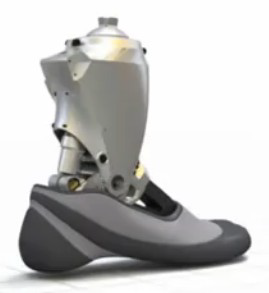
\includegraphics[width=\textwidth]{images/prot_01}

\textit{Centrifugeuse humaine développée par le CNRS / MEDES [1]} 

	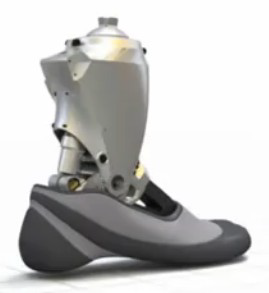
\includegraphics[width=\textwidth]{images/prot_01}

\textit{Modélisation cinématique} 

}%figues de la page de garde
\def\xxpied{%
Partie 3 -- Étude cinématique des systèmes  \\
Ch 5 : Cinématique du solide -- \xxactivite%
}

%---------------------------------------------------------------------------


\begin{document}
\chapterimage{png/Fond_Arch}
\pagestyle{empty}


\chapterimage{chapter_head_2.pdf}
%\chapterentete{}

\begin{tikzpicture}[remember picture,overlay]
\node at (current page.north west)
{\begin{tikzpicture}[remember picture,overlay]
\node[anchor=north west,inner sep=0pt] at (0,0) {\includegraphics[width=\paperwidth]{\thechapterimage}};
\draw[anchor=west] (-2cm,-6cm) node [line width=2pt,rounded corners=15pt,draw=ocre,fill=white,fill opacity=0.5,inner sep=40pt]{\strut\makebox[22cm]{}};
\draw[anchor=west] (1cm,-6cm) node {\huge\sffamily\bfseries\color{black} %
\begin{minipage}{1cm}
\rotatebox{90}{\LARGE\sffamily\textsc{\color{ocre}\textbf{\xxnumpartie}}}
\end{minipage} \hfill
\begin{minipage}[c]{14cm}
\begin{titrepartie}
\begin{flushright}
\renewcommand{\baselinestretch}{1.1} 
\Large\sffamily\textsc{\textbf{\xxpartie}}
\renewcommand{\baselinestretch}{1} 
\end{flushright}
\end{titrepartie}
\end{minipage} \hfill
\begin{minipage}[c]{3.5cm}
{\large\sffamily\textsc{\textbf{\color{ocre} \discipline}}}
\end{minipage} 
 };
\end{tikzpicture}};
\end{tikzpicture}

\vspace {3.5 cm}



\begin{tikzpicture}[remember picture,overlay]
\draw[anchor=west] (-2cm,-6cm) node {\huge\sffamily\bfseries\color{black} %
\begin{minipage}{2cm}
\LARGE\sffamily\textsc{\color{ocre}\textbf{\xxactivite}}
\end{minipage} \hfill
\begin{minipage}[c]{15cm}
\begin{titrechapitre}
\renewcommand{\baselinestretch}{1.1} 
\Large\sffamily\textsc{\textbf{\xxnumchapitre}}

\Large\sffamily\textsc{\textbf{\xxchapitre}}
\vspace{.5cm}

\renewcommand{\baselinestretch}{1} 
\normalsize\normalfont
\xxcompetences
\end{titrechapitre}
\end{minipage}  };
\end{tikzpicture}



\iftd
\else
\vfill

\begin{flushright}
\begin{minipage}[c]{.3\linewidth}
\begin{center}
\xxfigures
\end{center}
\end{minipage}\hfill
\begin{minipage}[c]{.6\linewidth}
\startcontents
\printcontents{}{1}{}
\end{minipage}
\end{flushright}
\newpage
\pagestyle{fancy}
\fi

%\newpage




\section{Avant propos}

\subsection{Notion de solide indéformable}
Lorsqu'un objet ou un système est soumis à des efforts, il peut subir, suivant la nature du matériau de grandes ou de petites déformations. 

\begin{exemple}
\begin{center}
\begin{tabular}{ccc}
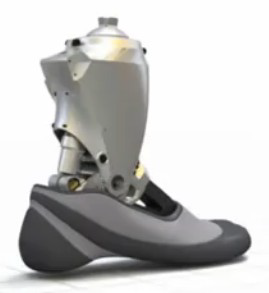
\includegraphics[width=.25\textwidth]{images/prot_01} & &
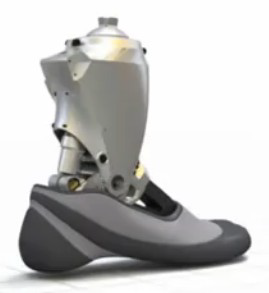
\includegraphics[width=.25\textwidth]{images/prot_01} \\
Pâte à modeler \cite{cite4}& &
%Nano gouttes d'or \cite{cite5} & 
Éprouvette de traction\\
\end{tabular}
\end{center}
\begin{itemize}
\item pale d'hélicoptère soumis à une force centrifuge;
\item fluides ...
\end{itemize}
\end{exemple}



Dans le cadre du programme de CPGE (PTSI et PT), plusieurs hypothèses peuvent être retenues.
En résistance des matériaux (programme de PT), ou lors des essais sur les matériaux (essai de traction par exemple), les matériaux sont considérés comme déformables. En effet, on observe la déformation de la matière au cours du temps.

En cinématique (PTSI), en statique (PTSI) et en dynamique (PT) les solides seront considérés comme indéformables. On considère en effet que les déformations sont négligeables par rapport aux études réalisées.

\begin{hypo}
\textbf{Solide indéformable}

%\begin{minipage}[c]{.6\linewidth}
%\ifthenelse{\boolean{prof}}{%
On considère deux points $A$ et $B$ d'un solide indéformable noté $S$. On note $t$ le temps.



\end{hypo}
\begin{rem}
En cinématique du solide indéformable, les fluides et les ressorts ne seront pas étudiés.
\end{rem}


\subsection{Notion de point appartenant à un solide}



\begin{warn}
En cinématique, il faudra vérifier si les points considérés sont bien des points matériels des solides considérés. 
\end{warn}



Dans le cas d'une roue de voiture, le point de contact entre la roue et le sol n'est pas un point matériel, il change au cours du temps...


... il en est de même pour le point de contact entre la came et le plateau.



Dans une transmission par engrenage simple, on modélise le contact entre $S_1$ et $S_2$ par un point qui est fixe par rapport au bâti. Ce point n'appartient ni au solide 1, ni au solide 2.



\section{Trajectoire d'un point appartenant à un solide}


\begin{defi}
\textbf{Trajectoire d'un point dans l'espace}

Soit un point $P$ se déplaçant dans un repère $\mathcal{R}_0 \left(O,\vect{i_0},\vect{j_0},\vect{k_0} \right)$. La trajectoire du point $P$ est définie par la courbe $\mathcal{C}(t)$ paramétrée par le temps $t$. On a : 
$$
\forall t\in \mathbb{R}^+, \vect{OP(t)}=
\left[
\begin{array}{l}
x(t)\\
y(t)\\
z(t)\\
\end{array}
\right]_{\mathcal{R}_0}
=x(t)\vect{i_0}+y(t)\vect{j_0}+z(t)\vect{k_0}
$$
\end{defi}


\begin{exemple}
\textit{Centrifugeuse}

Le paramétrage de la centrifugeuse est donnée ci dessous : 

\begin{minipage}[c]{.25\linewidth}
\begin{center}
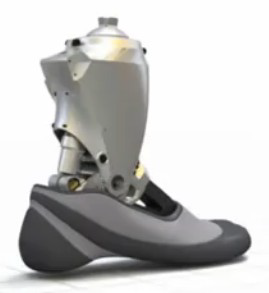
\includegraphics[height=3cm]{images/prot_01}
\end{center}
\end{minipage}\hfill
\begin{minipage}[c]{.45\linewidth}
\begin{center}
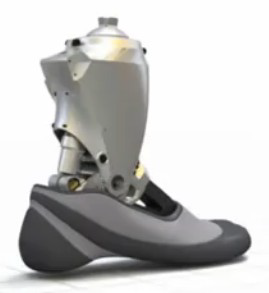
\includegraphics[height=3cm]{images/prot_01}
\end{center}
\end{minipage}\hfill
\begin{minipage}[c]{.25\linewidth}
Les paramètres constants du système sont les suivants : 
\begin{itemize}%[$\bullet$]
\item $\vect{O_0O_1} = a \vect{i_1}$
\item $\vect{O_1G} = b \vect{i_2} + c \vect{k_2}$
\end{itemize}
\end{minipage}

La trajectoire du point $G$ dans le repère $\mathcal{R}_0$  est donnée par le vecteur 
$$
\vect{O_0 G}(t)  = \vect{O_0O_1} + \vect{O_1G}
= a \vect{i_1} +  b \vect{i_2} + c \vect{k_2}
$$

Il faut alors projeter les vecteurs dans $\mathcal{R}_0$ : 
\begin{eqnarray*}
\vect{O_0 G}(t) &=& a \left(\cos\alpha(t) \vect{i_0} + \sin\alpha(t) \vect{j_0} \right) 
+ b \left(\cos\beta(t) \vect{i_1} - \sin\beta(t) \vect{k_1} \right) 
+ c\left(\cos\beta(t) \vect{k_1} + \sin\beta(t)\vect{i_1}\right)\\
&=& a \left(\cos\alpha(t) \vect{i_0} + \sin\alpha(t) \vect{j_0} \right) 
+ b \left(\cos\beta(t) \left(\cos\alpha(t) \vect{i_0} + \sin\alpha(t) \vect{j_0} \right) - \sin\beta(t) \vect{k_0} \right) \\
&& + c\left(\cos\beta(t) \vect{k_0} + \sin\beta(t)  \left(\cos\alpha(t) \vect{i_0} + \sin\alpha(t) \vect{j_0} \right) \right)\\
&=& \left[ \begin{array}{c} 
a \cos\alpha(t) + b \cos\beta(t) \cos\alpha(t) +c \sin\beta(t)\cos\alpha(t)\\
a \sin\alpha(t) + b \cos\beta(t) \sin\alpha(t) +c \sin\beta(t)\sin\alpha(t) \\
- b\sin\beta(t) + c\cos\beta(t)
\end{array}\right]_{\mathcal{R}_0}
\end{eqnarray*}

On a ainsi l'équation paramétrique de la position du point $G$.

\vspace{.25cm}

\end{exemple}
\section{Vitesse d'un point appartenant à un solide}

\subsection{Le vecteur vitesse}
\subsubsection{Définition}

\begin{defi}
\textbf{Vitesse d'un point appartenant à un solide}

Soit un solide $S_0$ auquel on associe le repère $\mathcal{R}_0$ $\left(O_0,\vect{i_0},\vect{j_0},\vect{k_0} \right)$.  Soit un solide $S_1$ auquel on associe le repère $\mathcal{R}_1$,  $\left(O_1,\vect{i_1},\vect{j_1},\vect{k_1} \right)$. Le solide $S_1$ est en mouvement par rapport au solide $S_0$. 

Soit un point $P$ appartenant au solide $S_1$. La vitesse du point $P$ appartenant au solide $S_1$ par rapport au solide $S_0$ se calcule donc ainsi : 
$$
\vect{V(P\in S_1/S_0)}(t) = \left[\dfrac{d\vect{O_0P(t)}}{dt}\right]_{\mathcal{R}_0}
$$
\end{defi}


\begin{warn}
\begin{minipage}[c]{.15\linewidth}
\begin{center}
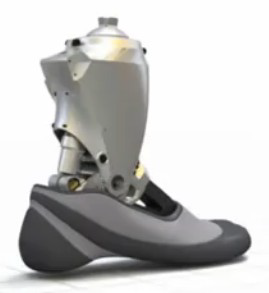
\includegraphics[width=.8\textwidth]{images/prot_01}
\end{center}
\end{minipage} \hfill
\begin{minipage}[c]{.8\linewidth}
\begin{itemize}
\item Attention à respecter rigoureusement la notation.
\item La vitesse dépend du point d'application.
\item Attention, << dériver un vecteur par rapport à une base >> est différent de << exprimer un vecteur dans une base>>.
\end{itemize}
\end{minipage}
\end{warn}


\begin{rem}
\begin{itemize}
\item $\vect{V(P\in S_1/S_0)}(t)$ dépend du temps $t$. On l'appelle vitesse instantannée. 
\item $\vect{V(P\in S_1/S_0)}(t)$ est tangent à la trajectoire du point $P$ dans $\mathcal{R}_0$.
\item $\vect{V(P\in S_1/S_0)}(t)$ peut s'exprimer dans n'importe quelle base.
\end{itemize}
\end{rem}


\subsubsection{Calcul du vecteur vitesse -- Application directe}

Soit un avion $S_1$ repéré par le repère $\mathcal{R}_1\left(O_1,\vect{i_1},\vect{j_1},\vect{k_1} \right)$ en mouvement libre par rapport à un repère $\mathcal{R}_0\left(O_0,\vect{i_0},\vect{j_0},\vect{k_0} \right)$.  La position de l'avion dans l'espace est repéré par le vecteur $\vect{O_0O_1}=x(t)\vect{i_0}+y(t)\vect{j_0}+z(t)\vect{k_0}$ ainsi que par les angles d'Euler.


Calculons la vitesse du point $O_1$ par rapport à $\mathcal{R}_0$ :
$$
\vectv{O_1}{S_1}{S_0} =  \left[\dfrac{d\vect{O_0 O_1}(t)}{dt}\right]_{\mathcal{R}_0} 
$$

\begin{rem}
Pour dériver le vecteur $\vect{O_0 O_1}(t)$ par rapport au repère $\mathcal{R}_0$ une méthode consiste en exprimer le vecteur $\vect{O_0 O_1}(t)$ dans $\mathcal{R}_0$ puis en dériver chacune des composantes. 
\end{rem}

\begin{eqnarray*}
\vectv{O_1}{S_1}{S_0} &=&  
\left[\dfrac{d\left(x(t)\vect{i_0}+y(t)\vect{j_0}+z(t)\vect{k_0} \right)}{dt}\right]_{\mathcal{R}_0}
= 
\left[\dfrac{d\left(x(t)\vect{i_0}\right)}{dt}\right]_{\mathcal{R}_0}
+\left[\dfrac{d\left(y(t)\vect{j_0}\right)}{dt}\right]_{\mathcal{R}_0}
+\left[\dfrac{d\left(z(t)\vect{k_0}\right)}{dt}\right]_{\mathcal{R}_0} \\
&=&
x(t)\left[\dfrac{d\vect{i_0}}{dt}\right]_{\mathcal{R}_0}
+ \dfrac{dx(t)}{dt} \vect{i_0}
+y(t)\left[\dfrac{d\vect{j_0}}{dt}\right]_{\mathcal{R}_0}
+ \dfrac{dy(t)}{dt} \vect{j_0}
+z(t)\left[\dfrac{d\vect{k_0}}{dt}\right]_{\mathcal{R}_0}
+ \dfrac{dz(t)}{dt} \vect{k_0} \\
%%&= &\dot{x(t)}\vect{i_0}+\dot{y(t)}\vect{j_0}+\dot{z(t)}\vect{k_0}
\end{eqnarray*}

On a : 
$$
\left[\dfrac{d\vect{i_0}}{dt}\right]_{\mathcal{R}_0} = 
\left[
\begin{array}{c}
\dfrac{d 1}{dt}\\
\dfrac{d 0}{dt}\\
\dfrac{d  0}{dt}\\
\end{array}
\right]_{\mathcal{R}_0}
 = \vect{0}
$$
Il est est de même pour $\left[\dfrac{d\vect{j_0}}{dt}\right]_{\mathcal{R}_0}$ et $\left[\dfrac{d\vect{k_0}}{dt}\right]_{\mathcal{R}_0}$.

\begin{rem}
\begin{itemize}
\item La dérivée d'un vecteur fixe $\vect{V}$ exprimé dans une base $\mathcal{B}_i$ par rapport à $\mathcal{B}_i$ est nul. Ainsi,  $\left[\dfrac{d\vect{i_i}}{dt}\right]_{\mathcal{R}_i}=\vect{0}$.
\item On note par un $\cdot$ la dérivée d'une fonction par rapport au temps : $\dfrac{dx(t)}{dt} = \dot{x}(t)$.
\end{itemize}

\end{rem}

Au final, on a donc :
$$\vectv{O_1}{S_1}{S_0} = \dot{x}(t) \vect{i_0}+\dot{y}(t) \vect{j_0}+\dot{z}(t) \vect{k_0} $$

\begin{exemple}
\textit{Centrifugeuse}

Calculer $\vectv{O_1}{S_1}{S_0}$.

Par définition, 
$$
\vectv{O_1}{S_1}{S_0} 
= \left[\dfrac{d\vect{O_0O_1}(t)}{dt}\right]_{\mathcal{R}_0}
= \left[\dfrac{d \left(a \vect{i_1}\right) }{dt}\right]_{\mathcal{R}_0}
= a \left[\dfrac{d  \vect{i_1} }{dt}\right]_{\mathcal{R}_0}
$$

On a :
\begin{eqnarray*}
\left[\dfrac{d  \vect{i_1} }{dt}\right]_{\mathcal{R}_0}
&=&\left[\dfrac{d \left(\cos\alpha(t)\vect{i_0}+\sin\alpha(t)\vect{j_0} \right)}{dt}\right]_{\mathcal{R}_0}
=\left[\dfrac{d  \cos\alpha(t)\vect{i_0}}{dt}\right]_{\mathcal{R}_0}
+\left[\dfrac{d  \sin\alpha(t)\vect{j_0} }{dt}\right]_{\mathcal{R}_0}\\
& = & 
\dfrac{d \cos\alpha(t)}{dt} \vect{i_0}  
+\cos\alpha(t)\underbrace{\left[\dfrac{d  \vect{i_0}}{dt}\right]_{\mathcal{R}_0}}_{\vect{0}}
+\dfrac{d \sin\alpha(t)}{dt} \vect{i_0}  
+\sin(t)\underbrace{\left[\dfrac{d  \vect{j_0}}{dt}\right]_{\mathcal{R}_0}}_{\vect{0}}\\
& = & -\dot{\alpha}(t)\sin\alpha(t) \vect{i_0}   + \dot{\alpha}(t)\cos\alpha(t) \vect{j_0}  = 
\dot{\alpha}(t)\vect{j_1}
\end{eqnarray*}

Ainsi,
$$
\vectv{O_1}{S_1}{S_0} 
= \left[\begin{array}{c} 
-a\dot{\alpha}(t)\sin\alpha(t) \\
a \dot{\alpha}(t)\cos\alpha(t) \\
0 \end{array}\right]_{\mathcal{R}_0}
=\left[\begin{array}{c} 0 \\ a\dot{\alpha}(t) \\ 0\end{array}\right]_{\mathcal{R}_1}
$$

Dans les deux cas, $\vect{O_0O_1}(t)$ est dérivé par rapport $\mathcal{R}_0$ mais il s'exprime différemment dans $\mathcal{R}_0$ et $\mathcal{R}_1$ :
\begin{itemize}
\item $\vectv{O_1}{S_1}{S_0} = -a\dot{\alpha}(t)\sin\alpha(t) \vect{i_0}   + a\dot{\alpha}(t) \cos\alpha(t) \vect{j_0}$ : ici la base de \textbf{projection} et de \textbf{dérivation} est la base $\mathcal{B}_0$;
\item $\vectv{O_1}{S_1}{S_0} = a\dot{\alpha}(t)\vect{j_1}$ : ici la base de dérivation est la base $\mathcal{B}_0$ et la base de projection est $\mathcal{B}_1$.
\end{itemize}

\end{exemple}


\begin{rem}
\begin{minipage}[c]{.65\linewidth}
Lorsqu'un point est confondu pour deux solides et qu'il n'y a pas de mouvement relatif entre les solides, (centre d'une liaison pivot ou d'une liaison rotule par exemple) les vitesses sont égales ainsi, ici : 
$$
\vect{V(0_1\in S_1/S_0)}(t) = \vect{V(0_1\in S_2/S_0)}(t)
$$

Par ailleurs, 
$$
\vect{V(0_1\in S_1/S_2)}(t) = \vect{0}
$$
\end{minipage}\hfill
\begin{minipage}[c]{.3\linewidth}
\begin{center}
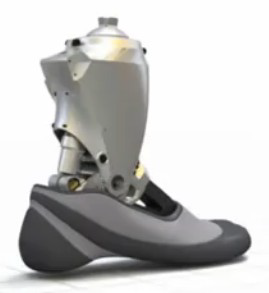
\includegraphics[width=.6\textwidth]{images/prot_01}
\end{center}
\end{minipage}
\end{rem}
\subsubsection{Détermination du vecteur vitesse dans les liaisons cinématiques}

\begin{resultat}
Lorsque il n'y a pas de degré de liberté de translation dans une liaison, la vitesse au centre de la liaison est nulle. Ainsi : 
\begin{itemize}
\item si les solides $S_1$ et $S_2$ sont en liaison rotule de centre $O$ alors $\vectv{O}{S_2}{S_1}=\vect{0}$;
\item si les solides $S_1$ et $S_2$ sont en liaison pivot de centre $O$ alors $\vectv{O}{S_2}{S_1}=\vect{0}$;
\item si les solides $S_1$ et $S_2$ sont en liaison rotule à doigt de centre $O$ alors $\vectv{O}{S_2}{S_1}=\vect{0}$.
\end{itemize}
\end{resultat}
\begin{exemple}
\textit{Centrifugeuse humaine}

Dans ce cas, on peut affirmer que :
$$
 \vectv{O_0}{S_1}{S_0} = \vect{0} \quad \text{et} \quad 
\vectv{O_1}{S_2}{S_1} = \vect{0}
$$
\textbf{Attention : dans le cas des liaisons pivots, ces relations ne sont vraies que sur les axes des liaisons et pour les mouvements relatifs entre les deux solides participant à la liaison.} 
\end{exemple}
\subsection{Vecteur instantané de rotation}

\subsubsection{Définition}

\begin{defi}
\textbf{Vitesse instantané de rotation entre deux solides -- Vecteur taux de rotation}

Soit un solide $S_0$ auquel on associe le repère $\mathcal{R}_0$ $\left(O_0,\vect{i_0},\vect{j_0},\vect{k_0} \right)$.  Soit un solide $S_1$ auquel on associe le repère $\mathcal{R}_1$,  $\left(O_1,\vect{i_1},\vect{j_1},\vect{k_1} \right)$. Le solide $S_1$ est en mouvement par rapport au solide $S_0$. 


Les rotations entre le solide $S_0$ et le solide $S_1$ sont paramétrés par les angles d'Euler $\psi(t)$, $\theta(t)$ et $\varphi(t)$.


\vspace{.25cm}

On appelle vecteur instantané de rotation entre les solides $S_0$ et $S_1$ le vecteur
$$
\vecto{S_1}{S_0} = \dot{\psi}(t) \vect{k_0} + \dot{\theta}(t) \vect{u} + \dot{\varphi}(t) \vect{k_1}
$$

$\dot{\psi}(t) $, $\dot{\theta}(t) $ et $\dot{\varphi}(t) $ sont en $rad/s$. 
\end{defi}

\begin{rem}

\begin{itemize}
\item On note sans distinction $\vecto{S_1}{S_0}$ et $\vecto{\mathcal{R}_1}{\mathcal{R}_0}$.
\item Le vecteur instantané de rotation est indépendant du point d'application.
\item On a la relation suivante :
$$\vecto{S_1}{S_0} = -\vecto{S_0}{S_1}$$
\end{itemize}
\end{rem}


\subsubsection{Détermination du vecteur vitesse instantané de rotation dans les liaisons cinématiques}

\begin{resultat}
Lorsqu'il n'y a pas de degrés de liberté de rotation dans une liaison ou que les degrés de liberté en rotation sont paramétrés, on a :  
\begin{itemize}
\item si les solides $S_1$ et $S_2$ sont en liaison pivot de centre $O$, d'angle $\alpha$ et d'axe $\vect{k}$ alors $\vecto{S_2}{S_1}=\dot{\alpha}\vect{k}$;
\item si les solides $S_1$ et $S_2$ sont en liaison glissière d'axe $\vect{z}$, $\vecto{S_2}{S_1}=\vect{0}$; 
\item si les solides $S_1$ et $S_2$ sont en liaison rotule de centre $O$,  et d'orientations $(\psi,\vect{k})$, $(\theta,\vect{u})$, $(\varphi,\vect{k_1})$, alors $\vecto{S_2}{S_1}=\dot{\psi}\vect{k}+\dot{\theta}\vect{u}+\dot{\varphi}\vect{k_1}$;
\item ...
\end{itemize}
\end{resultat}

\begin{exemple}
\textit{Centrifugeuse}

On a :
$$
\vecto{S_1}{S_0} = \dot{\alpha}\vect{k_0} 
\quad \quad
\vecto{S_2}{S_1} = \dot{\beta}\vect{j_1} 
$$

\end{exemple}
\subsection{Dérivation vectorielle -- Formule de Bour}


\begin{resultat}
\textbf{Dérivation vectorielle}

Soient $S_0$ et $S_1$ deux solides en mouvements relatifs et $\mathcal{R}_0$ et $\mathcal{R}_1$ les repères orthonormés directs associés. Soit $\vect{v}$ un vecteur de l'espace. On note $\vect{\Omega(\mathcal{R}_1/\mathcal{R}_0)}$ le vecteur instantané de rotation permettant d'exprimer les rotations entre chacune des deux bases. 

La dérivée d'un vecteur dans une base mobile se calcule donc ainsi :

$$
\left[\dfrac{d\vect{v}}{dt}\right]_{\mathcal{R}_0} =
\left[\dfrac{d\vect{v}}{dt}\right]_{\mathcal{R}_1} 
+ \vect{\Omega(\mathcal{R}_1/\mathcal{R}_0)}\wedge \vect{v}
$$
\end{resultat}

\begin{exemple}
\textit{Centrifugeuse}

Calcul de $\vectv{O_1}{S_1}{S_0}$.

On rappelle que :
$$
\vectv{O_1}{S_1}{S_0} 
= a \left[\dfrac{d  \vect{i_1} }{dt}\right]_{\mathcal{R}_0}
$$

Le calcul de $\left[\dfrac{d  \vect{i_1} }{dt}\right]_{\mathcal{R}_0}$ peut donc être réalisé ainsi : 
$$ 
\left[\dfrac{d  \vect{i_1} }{dt}\right]_{\mathcal{R}_0} = 
\underbrace{\left[\dfrac{d  \vect{i_1} }{dt}\right]_{\mathcal{R}_1}}_{\vect{0}} + \vecto{S_1}{S_0}\wedge \vect{i_1}
=\dot{\alpha}\vect{k_0}  \wedge \vect{i_1}
=\dot{\alpha} \vect{j_1}
$$

Ainsi 
$$
\vectv{O_1}{S_1}{S_0} 
= a \dot{\alpha} \vect{j_1}
$$
\end{exemple}


\subsection{Champ du vecteur vitesse dans un solide en mouvement}

\subsubsection{Mise en évidence}
Reprenons le cas d'un avion en déplacement dans le ciel . Soit $P$ un point appartenant à l'avion tel que $\vect{O_1P} = a\vect{i_1} + b\vect{j_1} + c\vect{k_1}$. 

Calculons la vitesse du point $P$ par rapport à $\mathcal{R}_0$ :

\begin{eqnarray*}
\vectv{P}{S_1}{S_0} & = &\left[\dfrac{d\vect{O_0 P}(t)}{dt}\right]_{\mathcal{R}_0}
= \left[\dfrac{d\left( \vect{O_0 O_1} + \vect{O_1P}\right)(t)}{dt}\right]_{\mathcal{R}_0} \\
&=&\vectv{O_1}{S_1}{S_0}+\left[\dfrac{d\vect{O_1 P}(t)}{dt}\right]_{\mathcal{R}_0} \\
\end{eqnarray*}

Calculons maintenant $\left[\dfrac{d\vect{O_1 P}(t)}{dt}\right]_{\mathcal{R}_0}$:
$$
\left[\dfrac{d\vect{O_1 P}(t)}{dt}\right]_{\mathcal{R}_0} = 
\left[\dfrac{d\vect{O_1 P}(t)}{dt}\right]_{\mathcal{R}_1} 
+ \vecto{S_1}{S_0} \wedge \vect{O_1 P}(t)
$$
$\vect{O_1 P}$ étant fixe dans le repère $\mathcal{R}_1$, $\left[\dfrac{d\vect{O_1 P}(t)}{dt}\right]_{\mathcal{R}_1}=\vect{0}$.

Au final, 
$$
\vectv{P}{S_1}{S_0} = \vectv{O_1}{S_1}{S_0}+
\vecto{S_1}{S_0} \wedge \vect{O_1 P}(t)
= \vectv{O_1}{S_1}{S_0}+
 \vect{P O_1}(t) \wedge \vecto{S_1}{S_0} 
$$
\subsubsection{Résultat}
\begin{resultat}
\textbf{Champ du vecteur vitesse dans un solide -- Formule de Varignon}

Soient $A$ et $B$ deux points appartenant à un solide $S_1$ en mouvement par rapport à $S_0$. Le champ des vecteurs vitesses est donc déterminé ainsi :
$$
\vect{V(B\in S_1/S_0)} = \vect{V(A\in S_1/S_0)} + \vect{BA}\wedge \vect{\Omega(S_1/S_0)}
$$
\end{resultat}

\begin{rem}

\textit{Moyen mnémotechnique}

\begin{minipage}[c]{.65\linewidth}
Comme la dérivée vectorielle, l'utilisation de cette formule est indispensable en mécanique en général et en cinématique en particulier.

On verra par la suite que le vecteur $\vect{\Omega}$ est appelé \textbf{R}ésultante du torseur cinématique. 

En conséquence, en utilisant le moyen mnémotechnique on a :
$$
\vect{V(\mathbf{B}\in S_1/S_0)} = \vect{V(\mathbf{A}\in S_1/S_0)} + \vect{\mathbf{BA}}\wedge \underbrace{\vect{\Omega(S_1/S_0)}}_{\mathbf{R}}
$$
\end{minipage}
\begin{minipage}[c]{.3\linewidth}
\begin{center}
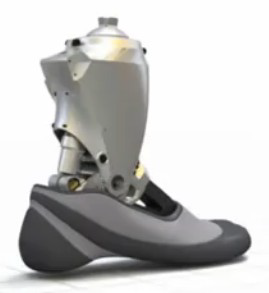
\includegraphics[width=.6\textwidth]{images/prot_01}
\end{center}
\end{minipage}
\end{rem}

\begin{rem}
\textit{Utilisation du champ de vecteur}

La formule du champ de vecteur est utilisée à chaque fois que la vitesse est connue en un point d'un solide et qu'on veut la calculer en un point appartenant à un autre point d'un même solide. 
\end{rem}

\begin{exemple}
\textit{Centrifugeuse}

Calcul de $\vectv{O_1}{S_1}{S_0}$.

$S_1$ et $S_0$ sont en liaison pivot de centre $O_0$, on a donc :  $\vectv{O_0}{S_1}{S_0}=\vect{0}$.

En conséquence, 
$$
\vectv{O_1}{S_1}{S_0} = \vectv{O_0}{S_1}{S_0} + \vect{O_1O_0}\wedge   \vecto{S_1}{S_0} = \vect{0} - a \vect{i_1} \wedge \left( \dot{\alpha}\vect{k_0} \right)
=a \dot{\alpha}\vect{j_1}
$$


\end{exemple}
\subsubsection{\'Equiprojectivité du champ des vecteurs vitesses}

\begin{resultat}
\textbf{Equiprojectivité}

Soit un solide $S_1$ en mouvement par rapport à un repère fixe $\mathcal{R}_0$. Soient deux points $A$ et $B$ appartenant au solide $S_1$. On démontre qu'à chaque instant $t$ :
$$
\vectv{A}{S_1}{\mathcal{R}_0}\cdot \vect{AB} = 
\vectv{B}{S_1}{\mathcal{R}_0}\cdot \vect{AB}
$$
\end{resultat}


\begin{py}

\begin{python}
TOTOTO
TOTOOT
if a<b :
    return none # Commentaire àaàaaà
    
oTOOTE
\end{python}
\end{py}

\begin{rem}
Cette propriété sera très utilisée en cinématique graphique lors de l'étude des mouvements plans.
\end{rem}


%\subsubsection{Détermination de la vitesse d'un point appartenant à un solide un mouvement -- Cas à un seul degré de liberté}
%Considérons notre avion en phase de décollage uniquement. Dans ces conditions et selon le paramétrage adopté,  $\theta(t)=\varphi(t)=0$. On a donc la figure de changement de base ci-contre.
%Soit $P$ un point appartenant à l'avion tel que $\vect{O_1P} = a\vect{i_1} + b\vect{j_1} + c\vect{k_1}$. 
%
%
%Calculons la vitesse du point $P$ par rapport à $\mathcal{R}_0$ :
%
%$$
%\vectv{P}{S_1}{S_0}=\left[\dfrac{d\vect{O_0 P}(t)}{dt}\right]_{\mathcal{R}_0}
%= \left[\dfrac{d\left( \vect{O_0 O_1} + \vect{O_1P}\right)(t)}{dt}\right]_{\mathcal{R}_0}
%=\underbrace{\left[\dfrac{d\vect{O_0 O_1}(t)}{dt}\right]_{\mathcal{R}_0}}_{\vectv{O_1}{S_1}{S_0}}
%+\left[\dfrac{d\vect{O_1 P}(t)}{dt}\right]_{\mathcal{R}_0}
%$$
%
%
%Calculons donc $\left[\dfrac{d\vect{O_1 P}(t)}{dt}\right]_{\mathcal{R}_0}$ :
%\begin{eqnarray*}
%\left[\dfrac{d\vect{O_1 P}(t)}{dt}\right]_{\mathcal{R}_0} & = & 
%\left[\dfrac{d\left(a\vect{i_1}+b\vect{j_1}+c\vect{j_1} \right)}{dt}\right]_{\mathcal{R}_0} \\
%& = & a\left[\dfrac{d\vect{i_1}}{dt}\right]_{\mathcal{R}_0}
%+ \underbrace{\left[\dfrac{da}{dt}\right]_{\mathcal{R}_0}}_{0} \vect{i_1}
%+b\left[\dfrac{d\vect{j_1}}{dt}\right]_{\mathcal{R}_0}
%+ \underbrace{\left[\dfrac{db}{dt}\right]_{\mathcal{R}_0}}_{0} \vect{j_1}
%+c\left[\dfrac{d\vect{k_1}}{dt}\right]_{\mathcal{R}_0} 
%+ \underbrace{\left[\dfrac{dc}{dt}\right]_{\mathcal{R}_0}}_{0} \vect{k_1} \\
%& = & a\left[\dfrac{d\vect{i_1}}{dt}\right]_{\mathcal{R}_0}
%+b\left[\dfrac{d\vect{j_1}}{dt}\right]_{\mathcal{R}_0}
%+c\left[\dfrac{d\vect{k_1}}{dt}\right]_{\mathcal{R}_0} \\
%\end{eqnarray*}
%
%Par ailleurs, d'après le paramétrage, $\vect{k_1}=\vect{k_0}$. En conséquences, 
%$\left[\dfrac{d\vect{k_1}}{dt}\right]_{\mathcal{R}_0} = \vect{0}$.
%
%
%Pour dériver les vecteurs $\vect{i_1}$, $\vect{j_1}$  dans la base $\mathcal{R}_0$ \textbf{une}\footnote{Mais pas forcément la meilleure.} des solutions est d'exprimer ces vecteurs dans $\mathcal{R}_0$. On a donc :
%
%\begin{eqnarray*}
%\vect{i_1} & = &  \cos\varphi(t) \vect{i_0} +  \sin\varphi(t) \vect{j_0}  \\
%\vect{j_1} & = &  \cos\varphi(t) \vect{j_0} -  \sin\varphi(t) \vect{i_0} 
%\end{eqnarray*}
%
%
%\begin{eqnarray*}
%\left[\dfrac{d\vect{i_1}}{dt}\right]_{\mathcal{R}_0} & = &  
%\dfrac{d\cos\varphi(t)}{dt} \vect{i_0} +  
%\cos\varphi(t)\left[\dfrac{d\vect{i_0}}{dt}\right]_{\mathcal{R}_0}
%\dfrac{d\sin\varphi(t)}{dt} \vect{j_0} + 
%\sin\varphi(t)\left[\dfrac{d\vect{j_0}}{dt}\right]_{\mathcal{R}_0}\\
%& = & -\dot{\varphi(t)}\sin\varphi(t) \vect{i_0} + \dot{\varphi(t)}\cos \varphi(t) \vect{j_0} \\
%& = & \dot{\varphi(t)}\left(  \cos \varphi(t) \vect{j_0} - \sin\varphi(t) \vect{i_0}\right)\\
%& = & \dot{\varphi(t)}\vect{j_1}\\
%\end{eqnarray*}
%
%De même :
%\begin{eqnarray*}
%\left[\dfrac{d\vect{j_1}}{dt}\right]_{\mathcal{R}_0} & = & - \dot{\varphi(t)}\vect{i_1}\\
%\end{eqnarray*}
%
%On a donc :
%$$
%\left[\dfrac{d\vect{O_1 P}(t)}{dt}\right]_{\mathcal{R}_0} = \dot{\varphi(t)}\left(a\vect{j_1}-b\vect{i_1}\right)
%$$
%
%Au final, 
%$$
%\vectv{P}{S_1}{S_0}=\vectv{O_1}{S_1}{S_0}
%+\dot{\varphi(t)}\left(a\vect{j_1}-b\vect{i_1}\right)
%$$


%\subsection{Champ des vecteurs vitesses des points d'un solide}

%\subsection{Calcul du vecteur vitesse}
%\begin{methode}

%\end{methode}

\section{Composition des mouvements}
\subsection{Composition du vecteur vitesse}
\begin{resultat}
\textbf{Composition du vecteur vitesse}
\label{ref_va}

Soit un solide $S_1$ en mouvement par rapport à un repère $\mathcal{R}_0$ et un solide $S_2$ par rapport au solide $S_1$. Pour chacun des points $A$ appartenant au solide $S_2$, on a :
$$
\vectv{A}{S_2}{\mathcal{R}_0}=
\vectv{A}{S_2}{S_1}+\vectv{A}{S_1}{\mathcal{R}_0}
$$
\end{resultat}

Démontrons ce résultat. $O_1$ est le centre de la liaison entre $\mathcal{R}_0$ et $S_1$. $O_1$ est donc fixe dans le repère $\mathcal{R}_0$. $O_2$ est le centre de la liaison entre $S_1$ et $S_2$. $A$ appartient à $S_2$. 
$$
\vectv{A}{S_2}{\mathcal{R}_0}
= \left[\dfrac{\vect{dO_1 A}}{dt}
\right]_{\mathcal{R}_0}
= \left[\dfrac{\vect{dO_1 O_2}}{dt}
\right]_{\mathcal{R}_0}
+
\left[\dfrac{\vect{dO_2 A}}{dt}
\right]_{\mathcal{R}_0}
=
\vectv{O_2}{S_1}{\mathcal{R}_0}
+
\left[\dfrac{\vect{dO_2 A}}{dt}\right]_{S_1}
+\vecto{S_1}{\mathcal{R}_0}\wedge \vect{O_2 A}
$$

$$
\vectv{A}{S_2}{\mathcal{R}_0}
=
\underbrace{\left[\dfrac{\vect{dO_2 A}}{dt}\right]_{S_1}}_{\vectv{A}{S_2}{S_1}}
+
\underbrace{\vectv{O_2}{S_1}{\mathcal{R}_0}
+
\vect{AO_2}
\wedge 
\vecto{S_1}{\mathcal{R}_0}}_{\vectv{A}{S_1}{\mathcal{R}_0}}
$$


On a donc bien : 
$$
\vectv{A}{S_2}{\mathcal{R}_0}
=
\vectv{A}{S_2}{S_1}
+
\vectv{A}{S_1}{\mathcal{R}_0}
$$

\begin{rem}
\begin{itemize}
\item $\vectv{A}{S_2}{\mathcal{R}_0}$ est appelé vecteur vitesse absolu;
\item $\vectv{A}{S_2}{S_1}$ est appelé vecteur vitesse relatif; 
\item $\vectv{A}{S_1}{\mathcal{R}_0}$ est appelé vecteur vitesse d'entraînement.
\end{itemize}
\end{rem}

\begin{resultat}
\textbf{Généralisation}

La décomposition du vecteur vitesse peut se généraliser avec $n$ solides : 
$$
\vectv{A}{S_n}{S_0}
=
\vectv{A}{S_n}{S_{n-1}}
+...+
\vectv{A}{S_1}{S_0}
$$

\end{resultat}

\subsection{Composition du vecteur instantané de rotation}
\begin{resultat}
\textbf{Composition du vecteur vitesse}

Soit un solide $S_1$ en mouvement par rapport à un repère $\mathcal{R}_0$ et un solide $S_2$ par rapport au solide $S_1$. On a : 
$$
\vecto{S_2}{\mathcal{R}_0}=
\vecto{S_2}{S_1}+\vecto{S_1}{\mathcal{R}_0}
$$
\end{resultat}

Pour démontrer ce résultat, prenons un vecteur $\vect{v}$ :
$$
\left[\dfrac{d\vect{v}}{dt}\right]_{S_1} = 
\left[\dfrac{d\vect{v}}{dt}\right]_{S_2} 
+ \vecto{S_2}{S_1} \wedge \vect{v}
$$

$$
\left[\dfrac{d\vect{v}}{dt}\right]_{S_1} = 
\left[\dfrac{d\vect{v}}{dt}\right]_{\mathcal{R}_0} 
+ \vecto{\mathcal{R}_0}{S_1} \wedge \vect{v}
$$

$$
\left[\dfrac{d\vect{v}}{dt}\right]_{\mathcal{R}_0} = 
\left[\dfrac{d\vect{v}}{dt}\right]_{S_2} 
+ \vecto{S_2}{\mathcal{R}_0} \wedge \vect{v} \Longleftrightarrow 
\left[\dfrac{d\vect{v}}{dt}\right]_{\mathcal{R}_0} 
-\left[\dfrac{d\vect{v}}{dt}\right]_{S_2} 
= \vecto{S_2}{\mathcal{R}_0} \wedge \vect{v}
$$

En faisant la soustraction des deux premières expressions on obtient : 
$$
\vect{0} = 
\left[\dfrac{d\vect{v}}{dt}\right]_{S_2} 
-\left[\dfrac{d\vect{v}}{dt}\right]_{\mathcal{R}_0} 
+ \vecto{S_2}{S_1} \wedge \vect{v}
- \vecto{\mathcal{R}_0}{S_1} \wedge \vect{v}
=\left[\dfrac{d\vect{v}}{dt}\right]_{S_2} 
-\left[\dfrac{d\vect{v}}{dt}\right]_{\mathcal{R}_0} 
+ \left(\vecto{S_2}{S_1} - \vecto{\mathcal{R}_0}{S_1}  \right)\wedge \vect{v}
$$

$$
\Longleftrightarrow
\left[\dfrac{d\vect{v}}{dt}\right]_{\mathcal{R}_0} 
-\left[\dfrac{d\vect{v}}{dt}\right]_{S_2} 
=
 \left(\vecto{S_2}{S_1} + \vecto{S_1}{\mathcal{R}_0}  \right)\wedge \vect{v}
$$
En utilisant la dernière relation on a donc : 
$$
\vecto{S_2}{\mathcal{R}_0} \wedge \vect{v}
=
 \left(\vecto{S_2}{S_1} + \vecto{S_1}{\mathcal{R}_0}  \right)\wedge \vect{v}
\Longleftrightarrow
\vecto{S_2}{\mathcal{R}_0} = \vecto{S_2}{S_1} + \vecto{S_1}{\mathcal{R}_0}
$$
\begin{proposition}
Toto
\end{proposition}

\begin{resultat}
\textbf{Généralisation}

La décomposition du vecteur instantané de rotation peut se généraliser avec $n$ solides : 
$$
\vecto{S_n}{S_0}
=
\vecto{S_n}{S_{n-1}}
+...+
\vecto{S_1}{S_0}
$$
\end{resultat}

\subsubsection{Exemple}

\begin{exemple}
\textit{Centrifugeuse}

Calcul de $\vectv{G}{S_2}{S_0}$.
%On a :
%$$\vecto{S_2}{S_0}=\vecto{S_2}{S_1}+\vecto{S_1}{S_0} = \dot{\alpha}\vect{k_0} + \dot{\beta}\vect{j_1}  $$

%Par ailleurs, 
On a : 
$$\vectv{G}{S_2}{S_0} = \vectv{G}{S_2}{S_1} + \vectv{G}{S_1}{S_0} $$
Calculons $\vectv{G}{S_1}{S_0}$ :
$$
\vectv{G}{S_1}{S_0} 
= \vectv{O_1}{S_1}{S_0} + \vect{GO_1}\wedge\vecto{S_1}{S_0}
= a\dot{\alpha}\vect{j_1} - \left(b\vect{i_2} + c\vect{k_2}\right) \wedge\left( \dot{\alpha} \vect{k_0}\right)
$$
$$
\vectv{G}{S_1}{S_0} 
= a\dot{\alpha}\vect{j_1}  + b\dot{\alpha} \sin(\beta+\pi/2) \vect{j_1} + c \dot{\alpha}\sin\beta\vect{j_1}
= \dot{\alpha} \left(a+b \cos\beta + c \sin\beta\right) \vect{j_1} 
$$

Par ailleurs calculons $\vectv{G}{S_2}{S_1}$ :
$$\vectv{G}{S_2}{S_1} = \vectv{O_1}{S_2}{S_1} + \vect{GO_1}\wedge \vecto{S_2}{S_1}
=-\left(b\vect{i_2}+c\vect{k_2}\right) \wedge \left(\dot{\beta}\vect{j_1}\right)
=-\dot{\beta}\left(b\vect{k_2}-c\vect{i_2} \right)
$$

Au final, 
$$\vectv{G}{S_2}{S_0} = \dot{\alpha} \left(a+b \cos\beta + c \sin\beta\right) \vect{j_1} 
-\dot{\beta}\left(b\vect{k_2}-c\vect{i_2} \right)
$$

Il est aussi possible de calculer $\vectv{G}{S_2}{S_0}$ ainsi : 
$$\vectv{G}{S_2}{S_0} = \left[\dfrac{d \vect{O_0G}}{dt}\right]_{\mathcal{R}_0}$$ 

\end{exemple}
\section{Accélération d'un point appartenant à un solide}
\subsection{Définition}
\begin{defi}
\textbf{Accélération d'un point appartenant à un solide}

Soit un solide $S_0$ auquel on associe le repère $\mathcal{R}_0$ $\left(O_0,\vect{i_0},\vect{j_0},\vect{k_0} \right)$.  Soit un solide $S_1$ auquel on associe le repère $\mathcal{R}_1$,  $\left(O_1,\vect{i_1},\vect{j_1},\vect{k_1} \right)$. Le solide $S_1$ est en mouvement par rapport au solide $S_0$. 


Soit un point $P$ appartenant au solide $S_1$. L'accélération du point $P$ appartenant au solide $S_1$ par rapport au solide $S_0$ se calcule donc ainsi : 
$$
\vect{\Gamma(P\in S_1/S_0)}(t) = \left[\dfrac{d\left( \vect{V(P\in S_1/S_0)}(t)\right)}{dt}\right]_{\mathcal{R}_0}
$$

\end{defi}



\subsection{Champ d'accélération d'un solide en mouvement}
On a vu que 
$\vectv{B}{S_1}{S_0} = \vectv{A}{S_1}{S_0} + \vect{BA} \wedge \vecto{S_1}{S_0}$. En dérivant cette expression on a donc : 
$$
\vectg{B}{S_1}{S_0} 
= \vectg{A}{S_1}{S_0} 
+\left[\dfrac{d\vect{BA}}{dt}\right]_{S_0} \wedge \vecto{S_1}{S_0}
+\vect{BA} \wedge \left[\dfrac{d\vecto{S_1}{S_0}}{dt}\right]_{S_0}
$$

$B$ et $A$ sont des points du solide $S_1$. On a donc : 
 $$
\left[\dfrac{d\vect{BA}}{dt}\right]_{S_0} =
\underbrace{\left[\dfrac{d\vect{BA}}{dt}\right]_{S_1}}_{\vect{0}} 
+ \vecto{S_1}{S_0} \wedge \vect{BA}
$$

$$
\vectg{B}{S_1}{S_0} 
= \vectg{A}{S_1}{S_0} 
+\vecto{S_1}{S_0} \wedge \vect{BA}
\wedge \vecto{S_1}{S_0}
+\vect{BA} \wedge \left[\dfrac{d\vecto{S_1}{S_0}}{dt}\right]_{S_0}
$$

$$
\vectg{B}{S_1}{S_0} 
= \vectg{A}{S_1}{S_0} 
+\vecto{S_1}{S_0} \wedge \vecto{S_1}{S_0}
\wedge \vect{AB}
+\left[\dfrac{d\vecto{S_1}{S_0}}{dt}\right]_{S_0} \wedge \vect{AB} 
$$

\begin{resultat}
Le champ des accélérations n'est donc pas un champ de moment.
\end{resultat}

\subsection{Composition des accélérations}


Au final, 
$$
\vectg{A}{S_2}{\mathcal{R}_0}
=
\vectg{A}{S_2}{S_1} + \underbrace{2\vecto{S_1}{\mathcal{R}_0}\wedge\vectv{A}{S_2}{S_1}}_{\vectg{A}{S_1}{\mathcal{R}_0}_{Cor}}
+\vectg{A}{S_1}{\mathcal{R}_0} 
$$


\begin{resultat}
On ne peut donc pas composer les accélérations.
On appelle : 
\begin{itemize}
\item $\vectg{A}{S_2}{\mathcal{R}_0}$ : accélération absolue;
\item $\vectg{A}{S_2}{S_1}$ : accélération relative;
\item $\vectg{A}{S_1}{\mathcal{R}_0}$ : accélération absolue;
\item $\vectg{A}{S_1}{\mathcal{R}_0}_{Cor}$ : accélération de Coriolis.
\end{itemize}
\end{resultat}

\section{Mouvements élémentaires}

En cinématique, les vitesses dépendront des dérivées des paramètres variables angulaires et linéaires. Pour les chaînes ouvertes, il sera nécessaire de disposer d'un actionneur par paramètre variable pour animer un système. Pour les chaînes fermées à une seule boucle, il suffira d'un actionneur en entrée du système pour l'animer.
%\begin{exemple}

%\end{exemple}
Les lois d'évolution des actionneurs sont au choix du concepteur du système. 

\subsection{Loi de vitesse uniforme}
Dans le cas où la vitesse est uniforme, on a la loi suivante : 



\subsection{Loi de vitesse en trapèze}
Physiquement il est impossible de passer d'une vitesse nulle à une vitesse non nulle. Par une première approche, il est possible qu'un actionneur soit piloté par une loi de vitesse en trapèze :





\begin{thebibliography}{2}
\bibitem[1]{cite1} Centrifugeuse humaine -- CNRS Photothèque/Sébastien Godefroy et MEDES, \textit{Avio et Tiger}, \url{http://www.medes.fr/home_fr/fiche-centrifugeuse/mainColumnParagraphs/0/document/Presentation%20centrifugeuse%2018.12.07.pdf}.
\bibitem[2]{cite4} Wallace et Gromit, \url{http://www.wallaceandgromit.com/goodies/}.
\bibitem[3]{JPP} Jean-Pierre Pupier -- Vitesse et accélération -- Dérivée vectorielle -- Mouvement de solides -- PTSI -- Lycée Rouvière Toulon.
\bibitem[4]{FM} Florestan Mathurin, \textit{Champs des Vecteurs Vitesse des Points d’un Solide}, cours de PCSI / MPSI du lycée Bellevue de Toulouse, \url{http://florestan.mathurin.free.fr} .
\end{thebibliography}
\end{document}

